\documentclass[a4,12pt]{horizon-theme}
\usepackage{lipsum}
\usepackage{fontawesome5}
\usepackage{graphicx,url}
\usepackage{float}
\usepackage{amsmath}
\usepackage{booktabs}
\usepackage{makecell}
\usepackage{array}
\usepackage{multirow}
\usepackage{caption}
\usepackage{subcaption}
\usepackage{siunitx}
\usepackage{enumitem}
\usepackage{gensymb}
\usepackage{csvsimple}
% \usepackage{tabularray}
\usepackage{stackengine}
\usepackage{xcolor, colortbl}
\usepackage{caption}
\usepackage[round]{natbib}
% \usepackage{longtable}


\strutlongstacks{T}

\setFiguresPath{.}
\setTitle{Decomposição LU para Matrizes Tridiagonais Cíclicas}
\setUniversity{Universidade de São Paulo}
\setFaculty{Escola Politécnica}
\setDepartment{MAP3121 - Métodos Numéricos e Aplicações}
\setCoverMainLogo{minerva.pdf}

\setCoverLeftBox{%
  {\Large Exercício Programa 01}\\[2pt]
  {Relatório Final}\\[45pt]
  {\large Natanael Magalhães Cardoso, 8914122}\\[5pt]
  {\large Valber Marcelino Filho, 11353165}\\[40pt]
  {\normalsize Professora: }{\large Cláudia Peixoto}\\[5pt]
  {\normalsize Turma: }{\large 03}
}

\renewcommand{\thefootnote}{\fnsymbol{footnote}}
\setCompactAuthors{Natanael Magalhães Cardoso\footnote{nUSP: 8914122, Turma: 03}, Valber Marcelino Filho\footnote{nUSP: 11353165, Turma: 03}}


\setHeaderRight{Escola Politécnica}
\setHeaderLeft{MAP3121 - Métodos Numéricos e Aplicações}



\begin{filecontents*}{a_n5_d4.csv}
i,a,b,c,d,x
1,{\bf 0.0000},2.0000,0.7500,0.9686,0.3827
2,0.3750,2.0000,0.6250,0.5358,0.2709
3,0.4167,2.0000,0.5833,-0.6374,-0.2392
4,0.4375,2.0000,0.5625,-0.6374,-0.4660
5,0.9000,2.0000,{\bf 0.0000},1.0000,0.7097
\end{filecontents*}

\begin{filecontents*}{c_n250_d10_truncated.csv}
i,a,b,c,d,x
1,0.2500000000,2.0000000000,0.7500000000,0.9917900138,0.3086835218
2,0.3750000000,2.0000000000,0.6250000000,0.8713187041,0.3221924507
3,0.4166666667,2.0000000000,0.5833333333,0.4047833431,0.1778839713
...,...,...,...,...,...
248,0.4989919355,2.0000000000,0.5010080645,0.9949912944,0.3317989975
249,0.4989959839,2.0000000000,0.5010040161,0.9987420027,0.3330519735
250,0.9980000000,2.0000000000,0.0020000000,1.0000000000,0.3334737509
\end{filecontents*}

\begin{filecontents*}{big_table.csv}
i,a,b,c,d,x_a,np_a,x_c,np_c
1,{\bf 0.250000},2.000000,0.750000,0.999877,0.378440,0.378440,0.330315,0.330315
2,0.375000,2.000000,0.625000,0.998027,0.323996,0.323996,0.333698,0.333698
3,0.416667,2.000000,0.583333,0.990024,0.332990,0.332990,0.330821,0.330821
4,0.437500,2.000000,0.562500,0.968583,0.324077,0.324077,0.324586,0.324586
5,0.450000,2.000000,0.550000,0.923880,0.310661,0.310661,0.310538,0.310538
6,0.458333,2.000000,0.541667,0.844328,0.284951,0.284951,0.284981,0.284981
7,0.464286,2.000000,0.535714,0.718126,0.243765,0.243765,0.243757,0.243757
8,0.468750,2.000000,0.531250,0.535827,0.183489,0.183489,0.183491,0.183491
9,0.472222,2.000000,0.527778,0.294040,0.102745,0.102745,0.102744,0.102744
10,0.475000,2.000000,0.525000,0.000000,0.003606,0.003606,0.003606,0.003606
11,0.477273,2.000000,0.522727,-0.323917,-0.106697,-0.106697,-0.106697,-0.106697
12,0.479167,2.000000,0.520833,-0.637424,-0.214728,-0.214728,-0.214728,-0.214728
13,0.480769,2.000000,0.519231,-0.883766,-0.301138,-0.301138,-0.301137,-0.301137
14,0.482143,2.000000,0.517857,-0.998027,-0.343306,-0.343306,-0.343308,-0.343308
15,0.483333,2.000000,0.516667,-0.923880,-0.320983,-0.320983,-0.320975,-0.320975
16,0.484375,2.000000,0.515625,-0.637424,-0.224483,-0.224483,-0.224511,-0.224511
17,0.485294,2.000000,0.514706,-0.171929,-0.063964,-0.063964,-0.063864,-0.063864
18,0.486111,2.000000,0.513889,0.368125,0.126168,0.126168,0.125807,0.125807
19,0.486842,2.000000,0.513158,0.818150,0.285825,0.285825,0.287136,0.287136
20,0.975000,2.000000,{\bf 0.025000},1.000000,0.360660,0.360660,0.355892,0.355892
\end{filecontents*}




\begin{document}
\horizonCover

\horizonTitle

\renewcommand{\thefootnote}{\arabic{footnote}}
\hspace{40pt}




\section{Introdução}
Uma matriz tridiagonal é uma matriz em banda que possui termos diferentes de zeros apenas na diagonal principal, na subdiagonal (abaixo da diagonal principal) e na supradiagonal (acima da diagonal principal). Como existem aplicações onde se é necessário resolver sistemas lineares com esse tipo de matrizes, uma  técnica numérica de resolução desses sitemas é a fatoração LU \citep{bana1, bana2}, que consiste na decomposição da matriz dos coeficientes do sistema em uma matriz triangular superior em outra inferior, que podem ser interpretadas como as matrizes provenientes da eliminação gaussiana. A triangular superior com a informação do resultado da eliminação e a triangular inferior com a informação dos multiplicadores. Além de sistemas lineares, a decomposição LU também é um passo fundamental para inversão de matrizes e para o cálculo de determinantes.

Sistemas tridiagonais são encontrados em problemas em diversas áreas, como em engenharia elétrica, na resolução de certos tipos de circuitos RLC \citep{ex1}, em economia, na criação de modelos estatísticos que utilizam a autoregressão de primeira ordem para induzir dependência na estrutura de covariância \citep{ex2}, e em oceanografia, na modelagem da propagação do som no oceano \citep{ex3}.

Nesse trabalho, implementamos o algoritmo para a decomposição LU de uma matriz tridiagonal e para a resolução de um sistema linear tridiagonal cíclico ou não cíclico usando a decomposição LU da matriz dos coeficientes do sistema.

Na Seção \ref{sec:metodo}, descrevemos o funcionamento do algorítmo implementado, incluindo instruções de execução, e na Seção \ref{sec:resultados}, comparamos o resultado do nosso algorítmo com outra biblioteca de álgebra linear e, também, analisamos ordem do algorítmo implementado. Por fim, concluímos que é possível implementar um algorítmo de solução de sistemas lineares de ordem $\mathcal{O}(n)$ considerando a tridiagonalidade da matriz dos coeficientes do sistema, que é consideravelmente menor que a ordem $\mathcal{O}(n^3)$ da eliminação gaussiana.


\section{Métodos}
\label{sec:metodo}

Este programa foi implementado usando a linguagem de programação Python \citep{python} e o pacote de computação científica Numpy \citep{numpy}, ambos de código aberto.

A descrição da implementação é dividida em duas partes: \emph{backend} (Seção \ref{sec:backend}) e \emph{frontend} (Seção \ref{sec:frontend}). A primeira descreve o functionamento do algorítmo de solução de sistemas tridiagonais cíclicos e a segunda descreve o funcionamento da interface do programa com o usuário.

\subsection{BackEnd}
\label{sec:backend}

O objetivo deste programa é encontrar a solução do sistema $Ax = d$, em que $A$ tem a forma descrita pela eq. \eqref{eq:matriz_A}. Isto é, encontrar os valores da matriz coluna $x$.

\begin{equation}\label{eq:matriz_A}
  A =
  \begin{bmatrix}
    b_1 & c_1 &        &        &        &         &         & a_1     \\
    a_2 & b_2 & c_2                                                    \\
        & a_3 & b_3    & c_3                                           \\
        &     & \ddots & \ddots & \ddots                               \\
        &     &        & a_i    & b_i    & c_i                         \\
        &     &        &        & \ddots & \ddots  & \ddots            \\
        &     &        &        &        & a_{n-1} & b_{n-1} & c_{n-1} \\
    c_n &     &        &        &        &         & a_n     & b_n     \\
  \end{bmatrix}_{n \times n}
\end{equation}

Uma matriz $A$ desta forma é chamada matriz tridiagonal em banda. Sua característica é que apenas os elementos das diagonais principal, subdiagonal e supradiagonal são diferentes de zero. Ela também pode ser dividida em cíclica, caso $a_1 \neq 0$ e $c_n \neq 0$, ou não cíclica, caso $a_1 = 0$ e $c_n = 0$.

Somente $3n$ dos elementos da matriz são, de fato, relevantes nos cálculos da solução do sistema, sendo $3n-2$ elementos diferentes de zero para o caso não cíclico. Então, para otimizar os recursos computacionais gastos, apenas os elementos da banda tridiagonal e das bordas são armazenados no programa, ao invés da matriz $A$ inteira. Dessa forma, a matriz $A$ é representada por três vetores: ${\bf a}=[a_i]_n$, ${\bf b}=[b_i]_n$ e ${\bf c}=[c_i]_n$, ambos de dimensão $n$. Para o caso não cíclico, os elementos $a_1$ e $c_n$ valem zero.


% \begin{equation}\label{eq:LU}
%     L = 
%     \begin{bmatrix}
%         l_1\\
%         l_2 & l_2\\
%             & l_3 & l_3\\
%             & & \ddots & \ddots\\
%             & & & l_{n-1} & l_{n-1}\\
%             & & & & l_n & l_n\\
%     \end{bmatrix}_{n \times n}
%     \qquad \textrm{e} \qquad U = 
%     \begin{bmatrix}
%         1 & u_1\\
%           & 1 & u_2\\
%           & & 1 & u_3\\
%           & & & \ddots & \ddots\\
%           & & & & 1 & u_{n-1}\\
%           & & & & & 1\\
%     \end{bmatrix}_{n \times n}
% \end{equation}

% \subsubsection{Sistemas Tridiagonais}

% \subsubsection{Decomposição LU}

% \subsubsection{Método de Crout}

% \subsubsection{Sistemas Tridiagonais Cíclicos}

% \subsubsection{Implementação}


Para encontrar a solução de um sistema tridiagonal, o programa calcula a decomposição LU da matriz dos coeficientes $A$ e, então, são calculadas as soluções para os sistemas $Ly = d$ e $Ux = y$, onde $x$ é a solução do sistema inicial $Ax = d$.

E, quando a matriz dos coeficientes $A$ é tridiagonal cíclica, o problema é separado em partes menores. É criada uma submatriz de $A$ de dimensão $m \times m$, com $m = n-1$, denominada $A'$, que é tridiagonal não cíclica. Com isso, são resolvidos dois sistemas tridiagonais não cíclicos: $A'y' = d'$ e $A'z' = v'$, onde $d' = (d_1, d_2, ..., d_m)^T$ e $v' = (c_n, 0, ..., 0, a_n)^T$.

Como dois sistemas tridiagonais com a mesma fatoração LU da matriz $A$ precisam ser resolvidos na implementação da solução do sistema tridiagonal cíclio, reutilizamos a fatoração LU para otimizar a performance do programa. A Tabela \ref{tab:func} mostra uma breve descrição para cada uma das três funções implementadas no \emph{backend}.

\begin{table}[!ht]
  \renewcommand\arraystretch{1.45}
  \centering
  \caption{Descrição dos argumentos da Interface de Linha de Comando}
  \label{tab:func}
  \doubleRuleSep
  \begin{tabular}{rp{0.7\textwidth}}
    \doubleTopRule
    Função                      & Descrição                                                                                                                                                                                                                                                                                                                     \\
    \midrule
    \texttt{decomp\_lu}         & Recebe a matriz $A$ na forma dos três vetores ${\bf a}$, ${\bf b}$ e ${\bf c}$, calcula a decomposição LU da matriz e retorna dois vetores, ${\bf l}$ e ${\bf u}$, que representam a matriz L e U da decomposição, respectivamente.                                                                                           \\
    \texttt{solve\_tridiagonal} & Recebe a decomposição LU da matriz dos coeficientes $A$ e o vetor ${\bf d}$ com os termos idependentes, resolve os sistemas $Ly = d$  e $Ux = y$ e retorna a solução do segundo sistema, um vetor ${\bf x}$, que é, também, a solução do sistema $Ax = d$ ou $(LU)x = d$.                                                     \\
    \texttt{solve\_cyclic}      & Recebe a matriz $A$ na forma dos três vetores ${\bf a}$, ${\bf b}$ e ${\bf c}$ e o vetor ${\bf d}$ com os termos idependentes, executa o algorítmo de solução do sistema para o caso cíclico através de duas chamadas à função \texttt{solve\_tridiagonal} e retorna um vetor ${\bf x}$, que representa a solução do sistema. \\
    \doubleBottomRule
  \end{tabular}
\end{table}



\subsection{FrontEnd}
\label{sec:frontend}

O \emph{frontend} consiste na implementação de uma Interface de Linha de Comando (CLI), por onde o usuário final interage com o programa. Através dela, o usuário obtêm o resultado de acordo com os argumentos definidos no momento da chamada do programa. Mudando estes argumentos, o usuário consegue escolher o tipo de sistema (cíclico ou não-cíclico), ajustar o tamanho da matriz dos coeficientes, a quantidade de casas decimais exibidas ou, até mesmo, o formato de saída. A Tabela \ref{tab:parametros} descreve cada um desses argumentos.

\subsubsection{Exemplos de chamadas do programa}
\label{sec:exemplos}

\begin{enumerate}
  \item \texttt{python3 ep1.py -a}
  \item \texttt{python3 ep1.py -a -n 5}
  \item \texttt{python3 ep1.py -a -n 250 -d 10}
  \item \texttt{python3 ep1.py -c}
  \item \texttt{python3 ep1.py -c -n 5}
  \item \texttt{python3 ep1.py -c -n 250 -d 10}
\end{enumerate}


As chamadas (1), (2) e (3), que possuem o argumento \texttt{-a}, configuram o programa para resolver um problema com matriz tridiagonal não-cíclica. Enquanto que as chamadas (4), (5) e (6), que possuem o argumento \texttt{-c}, configuram o programa para resolver um sistema com matriz tridiagonal cíclica. Além disso, as chamadas (1) e (4) executam o programa com os valores padrões de \texttt{-n = 20} e \texttt{-d = 4}, já esses argumentos não foram especificados. As chamadas (2) e (5) executam o programa com uma matriz dos coeficientes de dimensão $5 \times 5$ (\texttt{-n 5}). E, as chamadas (3) e (6) executam o programa com uma matriz dos coeficientes de dimensão $250 \times 250$ (\texttt{-n 250}) e os resultados são exibidos com 10 casas decimais (\texttt{-d 10}). As Tabelas \ref{tab:a_n5_d4} e \ref{tab:c_n250_d10} da Seção \ref{sec:resultados} mostram a saída do programa para as chamadas (2) e (6), respectivamente.


\begin{table}[!b]
  \renewcommand\arraystretch{1.45}
  \centering
  \caption{Descrição dos argumentos da Interface de Linha de Comando}
  \label{tab:parametros}
  \doubleRuleSep
  \begin{tabular}{rp{0.82\textwidth}}
    \doubleTopRule
    Argumento                & Descrição                                                                                                                                                                                                                                                                                                                                                                                                                                                                              \\
    \midrule
    \texttt{-h}              & \textit{Opcional.} Exibe uma mensagem de ajuda com breve descrição dos argumentos do programa.                                                                                                                                                                                                                                                                                                                                                                                         \\
    \texttt{-a}              & \textit{Obrigatório$^{*}$.} Configura o programa para resolver um sistema tridiagonal não-cíclico (ou acíclico). Isto é, a matriz dos coeficientes carregada possui $a_1 = 0$ e $c_n = 0$ e o algorítmo usado para resolver este sistema é o de matrizes tridiagonais não cíclicas.                                                                                                                                                                                                    \\
    \texttt{-c}              & \textit{Obrigatório$^{*}$.} Configura o programa para resolver um sistema tridiagonal cíclico. A matriz dos coeficientes gerada possui $a_1 \neq 0$ e $c_n \neq 0$ e o algorítmo usado é o que considera matrizes cíclicas. \textbf{Importante:} ($^{*}$) Os argumentos \texttt{-a} e \texttt{-c} são obrigatórios, mas não podem ser usado em conjunto. Uma chamada do programa deve ter o parâmetro \texttt{-a} ou o parâmetro \texttt{-c}, mas não ambos e nem a ausência de ambos. \\
    \texttt{-n <N>}          & \textit{Opcional.} Este argumento possui um parâmetro $N$ que deve ser um número inteiro que representa a dimensão $N \times N$ da matriz dos coeficientes. Valor padrão: \texttt{20}                                                                                                                                                                                                                                                                                                  \\
    \texttt{-d <D>}          & \textit{Opcional.} Este argumento possui um parâmetro $D$ que configura o número de dígitos decimais a serem mostrados na resposta do programa. Valor padrão: \texttt{4}                                                                                                                                                                                                                                                                                                               \\
    \texttt{-\phantom{}-csv} & \textit{Opcional.} Configura a saída do programa para ser impressa no formato CSV. Este parâmetro foi criado por propósito de desenvolvimento, mas pode ser usado pelo usuário final. Valor padrão: \texttt{False}                                                                                                                                                                                                                                                                     \\
    \doubleBottomRule
  \end{tabular}
\end{table}

\newpage
\section{Resultados}
\label{sec:resultados}

\subsection{Saída do programa}
\label{sec:saida}

A saída do programa é uma tabela com 6 colunas e o número de linhas definido pelo argumento \texttt{-n} na chamada do programa, ou 20 caso não haja especificação do argumento \texttt{-n}. As colunas da saída do programa são as mesmas das Tabelas \ref{tab:a_n5_d4} e \ref{tab:c_n250_d10}, que são exemplos de saída para diferentes valores de \texttt{-n} e \texttt{-d}. No primeiro, \texttt{-n=5} e \texttt{-d} não foi especificado e, no segundo, \texttt{-n=250} e \texttt{-d=10}.

\begin{table}[!ht]
  \centering
  \caption{Exemplo de saída do programa para resolução do problema cíclico executado com os argumentos \texttt{-n=5} e \texttt{-d} não foi especificado}
  \label{tab:a_n5_d4}
  \doubleRuleSep
  \begin{tabular}{*{6}{c}}
    \doubleTopRule
    % \multicolumn{2}{c}{Entrada} & \multicolumn{4}{c}{Saída FF} & \multicolumn{4}{c}{Saída UC}\\
    % \cmidrule(lr){1-2}\cmidrule(lr){3-6}\cmidrule(lr){7-10}
    $i$       & $a_i$     & $b_i$      & $c_i$     & $d_i$    & $x_i$      \\
    \midrule
    \csvreader[late after line=\\]{a_n5_d4.csv}{}%
    {\csvcoli & \csvcolii & \csvcoliii & \csvcoliv & \csvcolv & \csvcolvi} %
    \doubleBottomRule
  \end{tabular}
\end{table}

\begin{table}[!ht]
  \centering
  \caption{Exemplo de saída do programa para resolução do problema cíclico executado com os argumentos \texttt{-n=250} e \texttt{-d=10}}
  \label{tab:c_n250_d10}
  \doubleRuleSep
  \begin{tabular}{*{6}{c}}
    \doubleTopRule
    % \multicolumn{2}{c}{Entrada} & \multicolumn{4}{c}{Saída FF} & \multicolumn{4}{c}{Saída UC}\\
    % \cmidrule(lr){1-2}\cmidrule(lr){3-6}\cmidrule(lr){7-10}
    $i$       & $a_i$     & $b_i$      & $c_i$     & $d_i$    & $x_i$      \\
    \midrule
    \csvreader[late after line=\\]{c_n250_d10_truncated.csv}{}%
    {\csvcoli & \csvcolii & \csvcoliii & \csvcoliv & \csvcolv & \csvcolvi} %
    \doubleBottomRule
  \end{tabular}
\end{table}


\subsection{Testes}
\label{sec:testes}

\begin{table}[!ht]
  \centering
  \caption{Comparação dos valores obtidos com o programa implementado com o numpy para matrizes diagonais cíclicas e não cíclicas. Os valores em negrito ($a_1$ e $c_{20}$) são diferentes para solução cíclica e não cíclica, estes mostrados são para solução cíclica}
  \label{tab:comparacao}
  \doubleRuleSep
  \begin{tabular}{*{9}{c}}
    \doubleTopRule
    {}        & \multicolumn{4}{c}{Entradas} & \multicolumn{2}{c}{Sol. (não cíclico)} & \multicolumn{2}{c}{Sol. (cíclico)}                                                                \\
    \cmidrule(lr){2-5}\cmidrule(lr){6-7}\cmidrule(lr){8-9}
    $i$       & $a_i$                        & $b_i$                                  & $c_i$                              & $d_i$    & $x_i$     & $x_i$ (np) & $x_i$       & $x_i$ (np) \\
    \midrule
    \csvreader[late after line=\\]{big_table.csv}{}%
    {\csvcoli & \csvcolii                    & \csvcoliii                             & \csvcoliv                          & \csvcolv & \csvcolvi & \csvcolvii & \csvcolviii & \csvcolix} %
    \doubleBottomRule
  \end{tabular}
\end{table}

A validação das soluções foi feita comparando o valor da solução do sistema dado pelo algorítmo implementado com o valor dado pelo módulo de álgebra linear do Numpy, mostrada na Tabela \ref{tab:comparacao}. Nela é mostrada as entradas $a_i$, $b_i$, $c_i$ e $d_i$ junto com as soluções do sistema não cíclico e do sistema cíclico de $n=20$ incógnitas dadas por esse algorítmo e pelo Numpy (coluna np).





\newpage
\subsection{Contagem das operações}
\label{sec:contagem}

\begin{table}[!ht]
  \centering
  \caption{Contagem de operações para cada uma das funções listadas na Tabela \ref{tab:func}}
  \label{tab:contagem}
  \doubleRuleSep
  \begin{tabular}{l*{3}{c}}
    \doubleTopRule
    Função                      & \# mul/div & \# adi/sub & total    \\
    \midrule
    \texttt{decomp\_lu}         & $2n-2$     & $n-1$      & $3n-3$   \\
    \texttt{solve\_tridiagonal} & $3n-2$     & $2n-2$     & $5n-4$   \\
    \texttt{solve\_cyclic}      & $9n-11$    & $6n-8$     & $15n-19$ \\
    \doubleBottomRule
  \end{tabular}
\end{table}

A Tabela \ref{tab:contagem} mostra a contagem de operações feitas pelo algorítmo. Além disso, foi feito um experimento para cálcular o tempo de execução do algorítmo de solução de sistemas cíclicos em fução do número $n$ de incógnitas. Este experimento foi feito em uma máquina com as seguintes especificações de software: S.O. Ubuntu 20.04 Kernel GNU Linux 5.13.0-39, Python 3.8.10 (CPython compilado com GCC 9.4.0 no Linux), Numpy 1.21.4 e as especificações de hardware mostradas na Figura \ref{fig:topologia}. O resultado desse experimento é mostrado na Figura \ref{fig:tempos}, onde cada ponto representa o tempo médio de 200 execuções para cada valor de $n$, a área sombreada respresenta a banda de $\pm 1\sigma$ em torno da média e a reta vermelha é uma regressão linear do tempo médio, que tem a expressão dada na eq. \ref{eq:reg} e coeficiente de determinação $R^2 \approx 0.99689$.

\begin{equation}\label{eq:reg}
  T(n) = 0.0040619n -0.2301847 \quad \rm{[ms]}
\end{equation}

\begin{figure}[!ht]
  \centering
  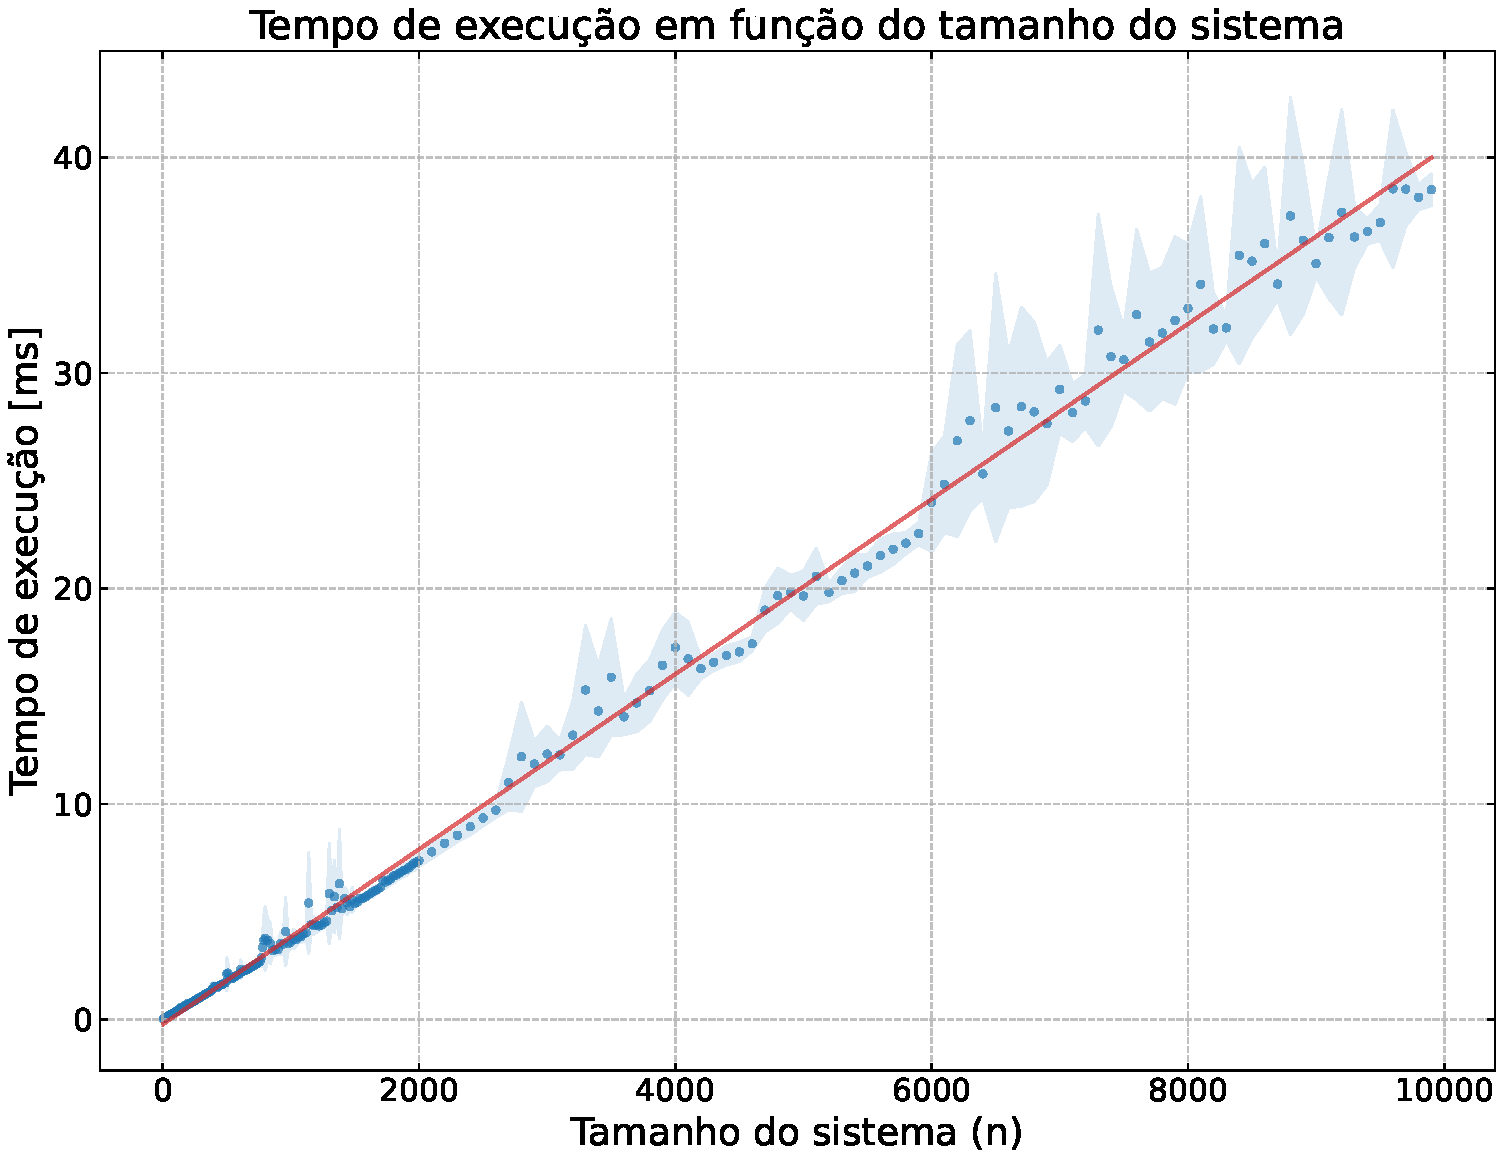
\includegraphics[width=0.88\textwidth]{../tempo.pdf}
  \caption{Tempo médio de execução em função do tamanho de sistemas cíclicos. Cada ponto representa a média de 200 execuções, a área sombreada representa $\pm 1\sigma$ da distribuição de execuções para cada $n$ e a reta vermelha é a regressão linear do tempo médio.}
  \label{fig:tempos}
\end{figure}


\section{Discussão e Conclusão}
\label{sec:conclusao}
Pela Tabela \ref{tab:contagem}, notamos que a contagem de operações do algorítmo de solução de sistemas cíclicos segue um polinômio de grau 1. A Figura \ref{fig:tempos}, que mostra o resultado experimental, confirma os cálculos teóricos. A partir da eq. \eqref{eq:reg} notamos que o tempo de execução possui escalamento linear em relação ao aumento do tamanho do sistema, $T(n) \in \mathcal{O}(n)$.

Com isso, concluímos que é possível implementar um algorítmo de complexidade $\mathcal{O}(n)$ em relação ao tempo para resolver um sistema tridiagonal cíclico usando decomposição LU. Este resultado representa uma vantagem significativa em relação aos métodos que não consideram a tridiagonalidade da matriz. O método da Eliminação Gaussiana, por exemplo, possui complexidade em relação ao tempo $\mathcal{O}(n^3)$ se não considerada a tridiagonalidade da matriz e $\mathcal{O}(n)$ se considerada \citep{ryaben}.

\vspace{10mm}

\section*{Apêndice}
\appendix

\begin{figure}[!ht]
  \centering
  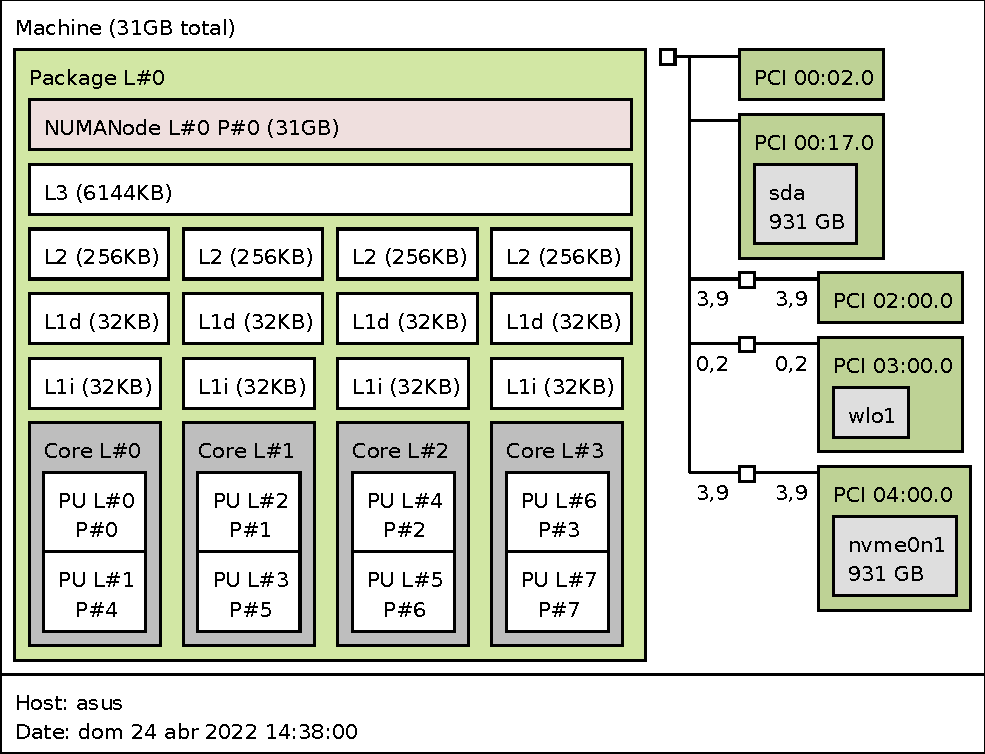
\includegraphics[width=\textwidth]{../topology.pdf}
  \caption{Topologia da máquina usada para testes experimentais criada pelo pacote open-source \texttt{hwloc} (\url{https://www.open-mpi.org/projects/hwloc/}).}
  \label{fig:topologia}
\end{figure}

\newpage

\bibliographystyle{plainnat}
\bibliography{refs}

\horizonBackCover
\end{document}
